\documentclass{standalone}
\usepackage{tikz}
\tikzset{>=latex} % for LaTeX arrow head
\usetikzlibrary{tikzmark} % for subnode
%\usepackage{pgfpages}
%\pgfpagesuselayout{resize to}[a4paper]

\begin{document}

\sffamily

% TIMELINE - Historical context
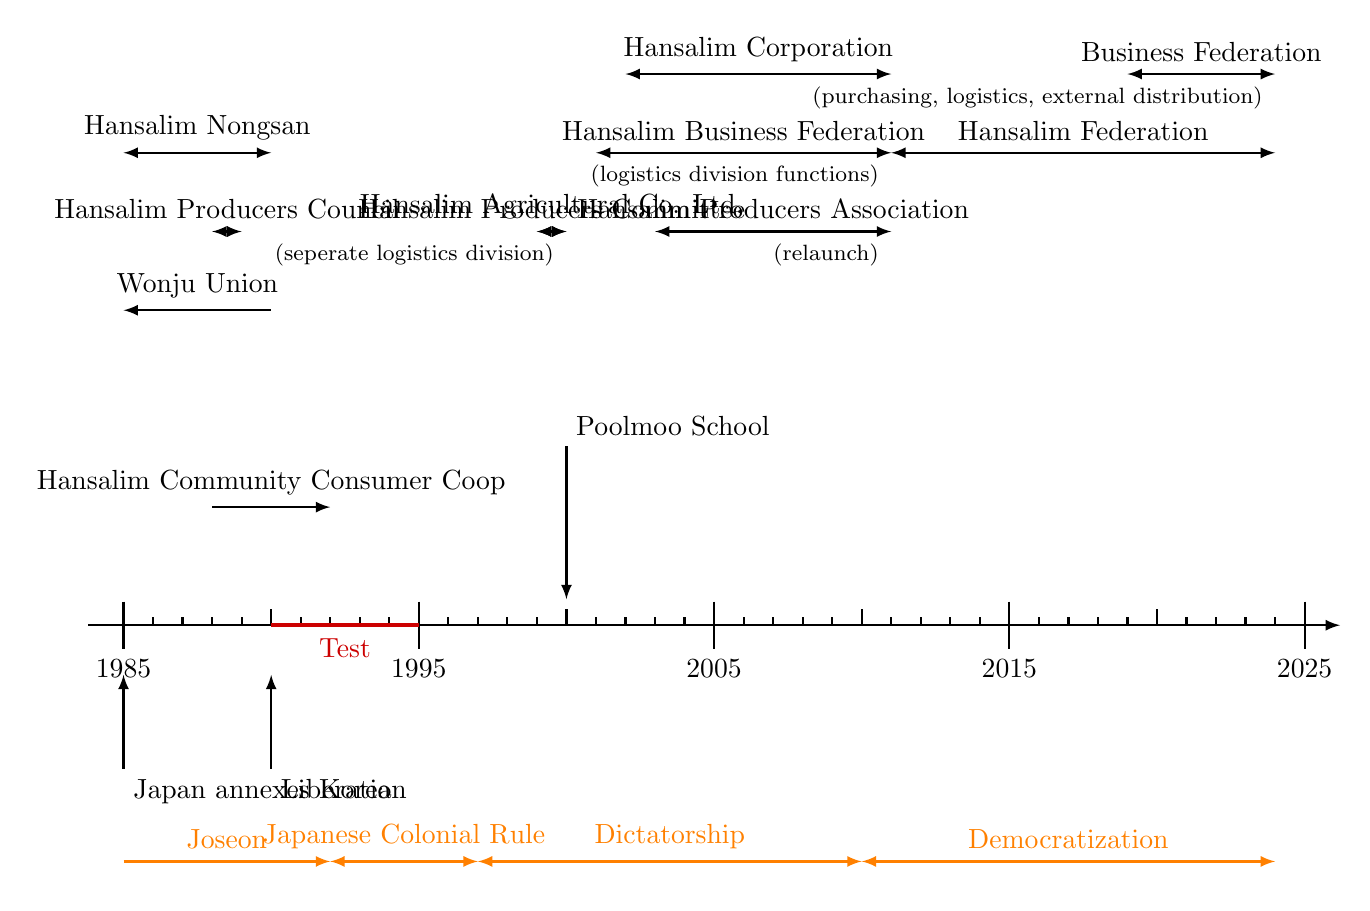
\begin{tikzpicture}[]
  % limits
  \newcount\yearOne; \yearOne=1985
  \def\w{15}    % width of axes
  \def\n{4}     % number of decades
  \def\lt{0.3} %  ten tick length
  \def\lf{0.2} % five tick length
  \def\lo{0.1} %  one tick length
  
  % help functions
  
        % Timeline labels
  \def\yearLabel(#1,#2){\node[above] at ({(#1-\yearOne)*\w/\n/10},\lt) {#2};}
        % Labelled arrows above and below timeline
  \def\yearArrowLabel(#1,#2,#3,#4){
    \def\xy{{(#1-\yearOne)*\w/\n/10}}; \pgfmathparse{int(#2*100)};
    \ifnum \pgfmathresult<0
      \def\yyp{{(\lt*(0.90+#2))}}; \def\yyw{{(\yyp-\lt*#3)}}
      \draw[<-,thick,black,align=center] (\xy,\yyp) -- (\xy,\yyw) node[below right=-0.2,black,align=left] at (\xy,\yyw) {#4};
    \else
      \def\yyp{{(\lt*(0.10+#2)}}; \def\yyw{{(\yyp+\lt*#3)}}
      \draw[<-,thick,black,align=center] (\xy,\yyp) -- (\xy,\yyw) node[above right=-0.2,black,align=left] at (\xy,\yyw) {#4};
    \fi}
    
        % Horizontal labelled arrows below or above timeline
  \def\yearSpan(#1,#2,#3,#4,#5,#6,#7){
      \def\from{{(#1-\yearOne)*\w/\n/10}};
      \def\to{{(#2-\yearOne)*\w/\n/10}};
      \def\height{{#5}};
        \draw[#6,thick,black!20!,color={#7}]
        (\from,\height) -- (\to,\height)
        node[below left=0.8pt,align=left] {#4}
        node[midway,above=0.8pt] {#3};
        }
        
        % Red labelled markers on the timeline itself
    \def\markerLabel(#1,#2,#3,#4){
        \def\from{{(#1-\yearOne)*\w/\n/10}};
        \def\to{{(#2-\yearOne)*\w/\n/10}};
        \def\height{{#4}};
            \draw[-,ultra thick,black!20!red]
            (\from,0) -- (\to,0)
            node[midway,below=#4] {#3};
    }
  
  % axis
  %\draw[thick] (0,0) -- (\w,0);
  \draw[->,thick] (-\w*0.03,0) -- (\w*1.03,0);
  
  % ticks
  \foreach \tick in {0,1,...,\n}{
    \def\x{{\tick*\w/\n}}
    \def\year{\the\numexpr \yearOne+\tick*10 \relax}
  	\draw[thick] (\x,\lt) -- (\x,-\lt) % ten tick
	             node[below] {\year};
	
	\ifnum \tick<\n
	  \draw[thick] ({(\x+\w/\n/2)},0) -- ({(\x+\w/\n/2)},\lf); % five tick
      \foreach \ticko in {1,2,3,4,6,7,8,9}{
        \def\xo{{(\x+\ticko*\w/\n/10)}}
  	    \draw[thick] (\xo,0) -- (\xo,\lo);  % one tick
	}\fi
  }
  
  % MARKERS
    \markerLabel(1990,1995,Test,0.8)
  
  % SITUATION
    %National Orgs
        \yearSpan(1985,1990,Hansalim Nongsan,\footnotesize{}\\
        \footnotesize{}\\
        \footnotesize{},6,<->,black)
        \yearSpan(2001,2011,Hansalim Business Federation,\footnotesize{(logistics division functions)}\\
        \footnotesize{}\\
        \footnotesize{},6,<->,black)
        \yearSpan(2002,2011,Hansalim Corporation,\footnotesize{}\\
        \footnotesize{}\\
        \footnotesize{},7,<->,black)
        \yearSpan(2011,2024,Hansalim Federation,\footnotesize{}\\
        \footnotesize{}\\
        \footnotesize{},6,<->,black)
        \yearSpan(2019,2024,Business Federation,\footnotesize{(purchasing, logistics, external distribution)}\\
        \footnotesize{}\\
        \footnotesize{},7,<->,black)

    %Production Organisation
        \yearSpan(1988,1989,{Hansalim Producers Council},\footnotesize{}\\
            \footnotesize{}\\
            \footnotesize{}\\
            \footnotesize{},5,<->,black)
            \yearSpan(1999,2000,{Hansalim Producers Committee},\footnotesize{}\\
            \footnotesize{}\\
            \footnotesize{}\\
            \footnotesize{},5,<->,black)
            \yearSpan(1999,2000,{Hansalim Agricultural Co. Ltd.},\footnotesize{(seperate logistics division)}\\
            \footnotesize{}\\
            \footnotesize{}\\
            \footnotesize{},5,<->,black)
            \yearSpan(2003,2011,{Hansalim Producers Association},\footnotesize{(relaunch)}\\
            \footnotesize{}\\
            \footnotesize{}\\
            \footnotesize{},5,<->,black)

    %SOCIAL MOVEMENTS & GRASS ROOTS ORGANIZATIONS
        \yearSpan(1988,1992,{Hansalim Community Consumer Coop},\footnotesize{}\\
            \footnotesize{},1.5,->,black)
    %Consumer Life co-ops
        \yearSpan(1985,1990,{Wonju Union},\footnotesize{}\\
            \footnotesize{}\\
            \footnotesize{}\\
            \footnotesize{}\\
            ,4,<-,black)

  % EVENTS
    \yearArrowLabel(1985,-3,4,Japan annexes Korea)
    \yearArrowLabel(1990,-3.0,4,Liberation)
    \yearArrowLabel(2000,1,6.5,Poolmoo School)
    %\yearArrowLabel(1960,1,5,Busan Credit Union)
    %\yearArrowLabel(1961,-3,4,Military Coup - Park Chung Hee)
    %\yearArrowLabel(1965,1,3.5,Organic farming movement)
    %\yearArrowLabel(1966,1,2,Wonju Credit Union)
    %\yearArrowLabel(1970,1,1,Korean Catholic Farmers Association)
    %\yearArrowLabel(1961,1.0,1.5,Nonghyup)
    %\yearArrowLabel(1987,1.0,1.5,Hansalim)
    
  %PERIODS
    \yearSpan(1985,1992,Joseon,,-3,->,orange)
    \yearSpan(1992,1997,Japanese Colonial Rule,,-3,<->,orange)
    \yearSpan(1997,2010,Dictatorship,,-3,<->,orange)
    \yearSpan(2010,2024,Democratization,,-3,<->,orange)
  
\end{tikzpicture}

\end{document}